\cotefile{10}
\scanpage{131}

b) Example of an exact faithful $\unsure{\otimes|\Omega}$ functor, compatible with $\deleted{\unsure{k\handwritten{\varphi}|k\handwritten{\psi}}}$ $1,\handwritten{\unsure{\varphi|\phi|\psi}},{}^{\handwritten{\unsure{\vee|\nu|v}}}$ (but not \deleted{with} $\handwritten{\unsure{\psi|\varphi|\mu}}$ !), and which is not locally isomorphic to the given fiber functor. - We take for $G$ a group. We then note that giving a system of $\deleted{\unsure{M|W}}\handwritten{L}_{g}$ and isomorphisms $(\unsure{\rlap{\(x\)}-|*})$ \deleted{, with $(\rlap{\(x\)}-\rlap{\(x\)}-)$}, satisfying the various compatibilities, is equivalent to giving an extension of $G$ by $k^{\handwritten{*}}$. The functor $\inserted{F'}$ is isomorphic to \unsure{\rlap{y}the|the|y} functor $F$ if and only if this extension splits. The set of isomorphism classes of fiber functors defined over $k$ is thus in 1-1 correspondence with $H^{2}(G,k^{\handwritten{*}})$. Now Even if $G$ is commutative (fo\unsure{\rlap{f}r|r|f} example the product of two isomorphic cyclic groups of order prime to \deleted{$k^{\handwritten{*}}$), and $k$} $\mathrm{car}.k$) and $k$ algebraically closed, the $H^{2}$ can be nonzero; \deleted{it is then not killed in} moreover a nonzero element of $H^{2}$ is killed in no extension of $k$ (if $k$ algebraically closed), by the principle of finite exten\unsure{\rlap{i}s\rlap{o}i\rlap{n}on|siion|sion}.

If however $G$ is commutative, and if we restrict ourselves to the $F'$ compatible with $\handwritten{\psi}$ as well, we find the commutative extensions of $G$ by $k^{\handwritten{*}}$; if $k$ is alg\unsure{\rlap{g}e|e}braically closed, hence $k^{\handwritten{*}}$ divisible, then every such extension splits, so $F'$ is then isomorphic to $F$ (in conf\rlap{i}ormity with the Galois theory relative to the case where the diagonal map of $U$ is commutative ...).

Thus, there can be fibre functors compatible with the given $\handwritten{\psi}$, and others which are not and which consequently are not locally isomorphic to the first. This therefore shows \margin{\handwritten{study the commutativity \unsure{\&|+} \unsure{associativity|associativity} constraints for gradings modulo 2.}} that \rlap{i}o\rlap{l}ne cannot neglect the \deleted{condition of} commutativity constraint as one would have liked to be able to do. Moreover, \margin{\figure{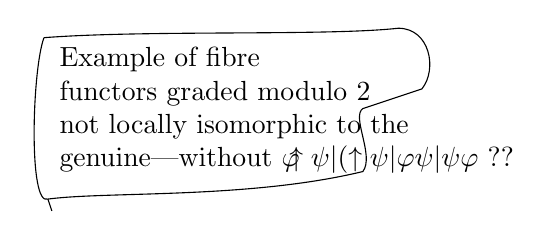
\begin{tikzpicture}[x=1cm,y=1cm]
\node[anchor=north west,align=left,inner sep=2pt] at (.12,-.05) {\handwritten{Example of fibre}\\\handwritten{functors graded modulo 2}\\\handwritten{not locally isomorphic to the}\\\handwritten{\unsure{genuine|without} $\unsure{\rlap{\(\varphi\)}\uparrow\psi|(\uparrow\psi|\varphi\psi|\psi\varphi}$ ??}};
\draw (0,0) .. controls (1.3,.1) and (3.6,.02) .. (4.5,.12) .. controls (4.9,.12) and (5,-.4) .. (4.8,-.65) -- (4.05,-.9) .. controls (3.9,-1) and (4.2,-1.5) .. (4.05,-1.7) .. controls (2.6,-2.05) and (.8,-1.95) .. (.05,-2.05) .. controls (-.2,-2.15) and (-.15,-.4) .. (0,0);
\draw (.05,-2.05)--(.1,-2.2);
\end{tikzpicture}}} this suggests that in the absence of a commutativity constraint, the classification of fiber functors is given by groups of the type of Brauer cohomology.

% archive sheet number: 130
